\subsection{Free Undamped Vibrations ($b = 0$)}
\noindent
In this case, our equation simplifies to
\begin{equation*}
	my^{\prime\prime} + ky = 0
\end{equation*}
The two roots of ou auxiliary equation are
\begin{equation*}
	r = \pm i \sqrt{\frac{k}{m}} = \pm i\omega
\end{equation*}
So, our solution becomes
\begin{equation*}
	y = C_1\cos{(\omega t)} + C_2\sin{(\omega t)}
\end{equation*}
This is the same $\omega$ from physics that means angular frequency, so the same physics formulas apply, like $T = \frac{2\pi}{\omega}$.\\

\noindent
We can simplify this a bit further. If we think of the $\cos$ and $\sin$ components as being sides of a right triangle like so,
\begin{center}
	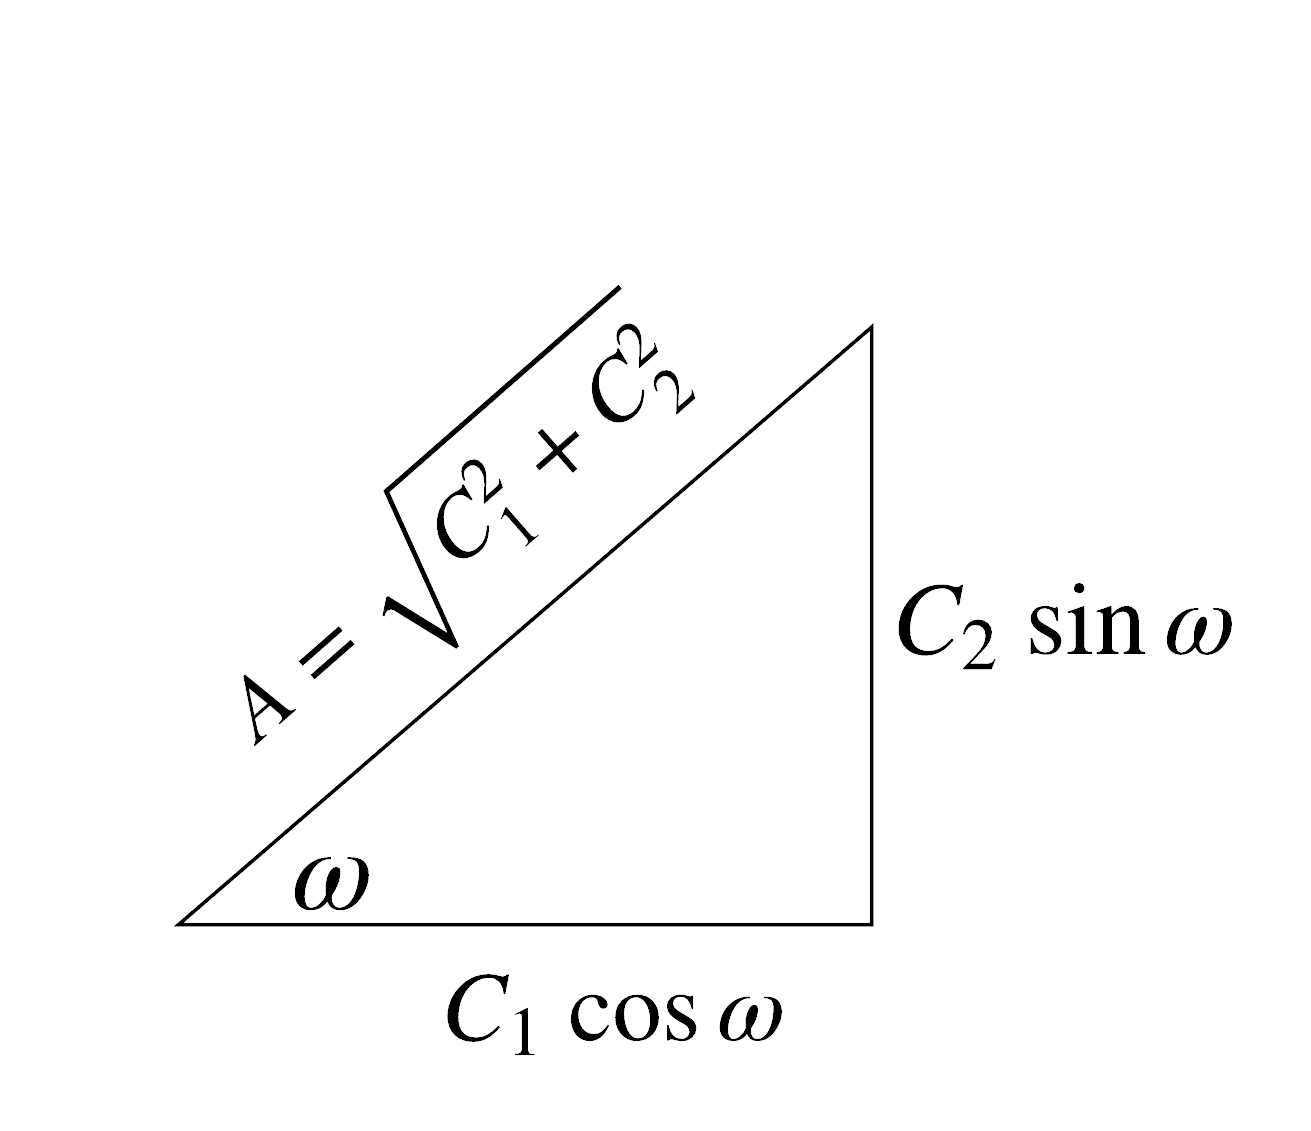
\includegraphics[width=0.5\textwidth]{./higherOrder/freeVibrs/triangle.png}
\end{center}
then we rewrite our equation as
\begin{equation*}
	y = A\left( \frac{C_1}{\sqrt{C_1^2 + C_2^2}}\cos{(\omega t)} + \frac{C_2}{\sqrt{C_1^2 + C_2^2}}\sin{(\omega t)} \right)
\end{equation*}
Note that since $\left(\frac{C_1}{A}\right)^2 + \left(\frac{C_2}{A}\right)^2 = 1$, we can rewrite these coefficients as $\cos{\phi}$ and $\sin{\phi}$ respectively where
\begin{equation*}
	\phi = \begin{cases}
		\arctan{(\frac{C_2}{C_1})} & C_1 > 0 \\
		\arctan{(\frac{C_2}{C_1})} + \pi & C_1 \leq 0
	\end{cases}
\end{equation*} 
So, our equation becomes
\begin{equation*}
	y = A\left(\cos{(\omega t)}\cos{\phi} + \sin{(\omega t)}\sin{\phi}\right)
\end{equation*}
Using the $\cos$ angle addition formula
\begin{equation*}
	y = A\cos{(\omega t - \phi)}
\end{equation*}
\begin{center}
	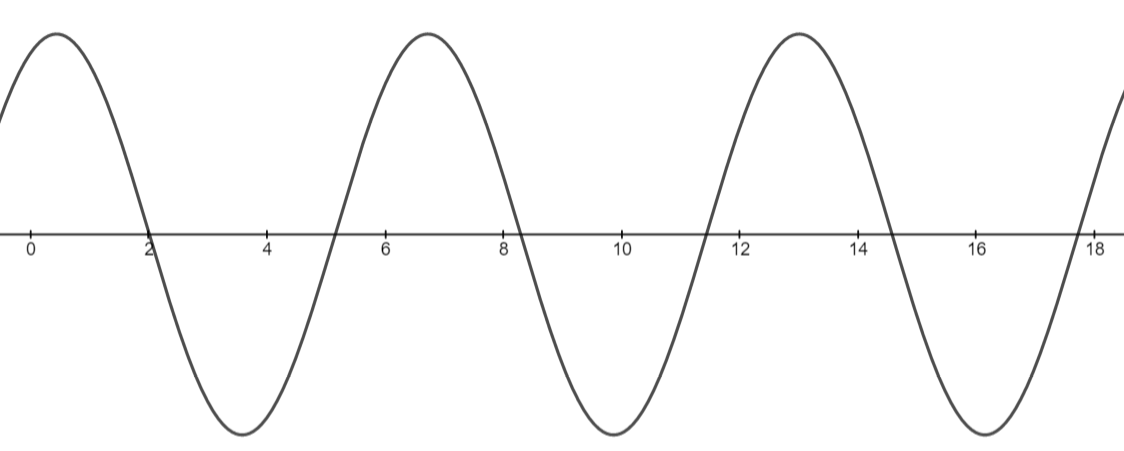
\includegraphics[width=0.5\textwidth]{./higherOrder/freeVibrs/undampedfree.png}
\end{center}
As we can see, an undamped free vibration will simply oscillate back and forth without decay.

\ifodd\includeHigherOrderExamples\begin{example}
	A 2kg mass in an undamped system is attached to a spring with $k = 50 \text{N/m}$. The initial position of the masss is $y_0 = -0.25\text{m}$. The initial velocity is $v_0 = -1\text{m/s}$. Find an expression for $y(t)$, the position of the mass at time $t$. Write your answer in terms of a $\cos$ and a phase shift. Find the period and frequency in proper units.
\end{example}
The IVP describing this problem is
\begin{equation*}
	\begin{cases}
		2y'' + 50y = 0 \\
		y'(0) = -1 \\
		y(0) = -0.25
	\end{cases}
\end{equation*}
Extracting the auxiliary equation and finding the roots,
\begin{equation*}
	2r^2 + 50 = 0 \implies r = \pm 5i
\end{equation*}
So, our general solution is
\begin{equation*}
	y = C_1\cos{(5t)} + C_2\sin{(5t)}
\end{equation*}
Solving for $C_1$ and $C_2$,
\begin{equation*}
	y(0) = -0.25 = C_1 \implies C_1 = -0.25
\end{equation*}
\begin{equation*}
	y' = -5C_1\sin{(5t)} + 5C_2\cos{(5t)}
\end{equation*}
\begin{equation*}
	y'(0) = -1 = 5C_2 \implies C_2 = -0.2
\end{equation*}
Solving for $\phi$, keeping in mind that $C_1 < 0$
\begin{equation*}
	\phi = \arctan{\frac{C_2}{C_1}} + \pi = \arctan{\frac{4}{5}} + \pi
\end{equation*}
So, our answer is (in units of meters)
\begin{equation*}
	y = \sqrt{(-0.25)^2 + (-0.2)^2}\cos{\left(5t - \arctan{\left(\frac{4}{5}\right)} - \pi\right)} \approx 0.32\cos{\left(5t - 3.82\right)}
\end{equation*}
Solving for the period,
\begin{equation*}
	T = \frac{2\pi}{\omega} = \frac{2\pi}{5} \text{s}
\end{equation*}
Solving for the frequency,
\begin{equation*}
	f = \frac{1}{T} = \frac{5}{2\pi} \text{Hz}
\end{equation*}\fi